\documentclass[default]{beamer}
\setbeamertemplate{navigation symbols}{}

\usetheme{CambridgeUS}
%\useoutertheme{infolines}
\usecolortheme{beaver}

\usepackage[utf8]{inputenc}					% Выбор языка и кодировки
\usepackage[english]{babel}	% Языки: русский, английский
\usepackage{csquotes}

\usepackage{tikz}
\usetikzlibrary{arrows,shapes,calc}
\everymath{\displaystyle}
\tikzstyle{every picture}+=[remember picture]

\usepackage{animate}
\usepackage{fp}
\usepackage{textpos}

\usepackage[
	language=auto,
	autolang=other,
	backend=biber,
	style=authortitle,
	sorting=ydnt,
	maxbibnames=5
]{biblatex}
\addbibresource{panov_bica2018.bib}
				
\DeclareSourcemap{
	\maps[datatype=bibtex, overwrite]{
		\map{
			\step[fieldset=langid, fieldvalue=english]
			\step[fieldset=doi, null]
			\step[fieldset=issn, null]
			\step[fieldset=isbn, null]
			\step[fieldset=url, null]
			\step[fieldsource=language, fieldset=langid, origfieldval]
		}
	}
}
\DeclareBibliographyDriver{std}{%
	\usebibmacro{bibindex}%
	\usebibmacro{begentry}%
	\usebibmacro{author/editor+others/translator+others}%
	\setunit{\labelnamepunct}\newblock
	\usebibmacro{title}%
	\newunit\newblock
	\usebibmacro{maintitle+booktitle}
	\newunit\newblock
	\usebibmacro{journal}%
	\newunit\newblock
	\usebibmacro{date}%
	\newunit\newblock
	\usebibmacro{finentry}
}
\DeclareBibliographyAlias{article}{std}
\DeclareBibliographyAlias{book}{std}
\DeclareBibliographyAlias{inproceedings}{std}
\DeclareBibliographyAlias{incollection}{std}

\graphicspath{{../../images/}} 			% Пути к изображениям

\makeatletter
\setbeamertemplate{footline}
{
	\leavevmode%
	\hbox{%
		\begin{beamercolorbox}[wd=.333333\paperwidth,ht=2.25ex,dp=1ex,center]{author
				in head/foot}%
			\usebeamerfont{author in
				head/foot}\insertshortauthor~~\beamer@ifempty{\insertshortinstitute}{}{(\insertshortinstitute)}
		\end{beamercolorbox}%
		\begin{beamercolorbox}[wd=.333333\paperwidth,ht=2.25ex,dp=1ex,center]{title in
				head/foot}%
			\usebeamerfont{title in head/foot}\insertshorttitle
		\end{beamercolorbox}%
		\begin{beamercolorbox}[wd=.333333\paperwidth,ht=2.25ex,dp=1ex,right]{date in
				head/foot}%
			\usebeamerfont{date in head/foot}\insertshortdate{}\hspace*{1em}
			\insertframenumber{}\hspace*{2ex} 
		\end{beamercolorbox}
	}%
	\vskip0pt%
}

\addtobeamertemplate{frametitle}{}{
	\begin{textblock*}{100mm}(\textwidth-35pt,-20pt)
		
\includegraphics[width=1.5cm]{misc/logos/frccsc.png}
	\end{textblock*}
}

\newcommand{\predmatr}[3]{
	\node[ell, rectangle, minimum height = 15, minimum width = 7.5]  at (#1 pt,#2 pt) {}; 
	\node[ellf, rectangle, minimum height = 15, minimum width = 7.5] at (#1+7.5 pt,#2 pt) {};
	\node[minimum height = 15, minimum width = 15] (#3) at (#1+3.3pt,#2 pt) {};
	\draw[ell] (#1+7.5 pt,#2+7.5 pt) -- (#1 +7.5 pt,#2-7.5 pt);
}
\renewcommand*{\bibfont}{\tiny}
\setlength\bibitemsep{-5pt}

\begin{document}
	
	\title[HTM$\rightarrow$HCN+Anomaly Detection]{Extended Hierarchical Temporal Memory for Motion Anomaly Detection}
	\author[Daylidyonok, Frolenkova, Panov]{Ilya Daylidyonok, Anastasiya Frolenkova, Alelsandr I. Panov}
	\institute[RAS]{Federal Research Center ``Computer Science and Control''\\Russian Academy of Sciences (RAS)\\Moscow Institute of Physics and Technolgy\\\textbf{Moscow}}
	\date[August 24 -- BICA 2018]{August 24 -- BICA 2018} 
		
	\begin{frame}
		\titlepage
		\centering
		
\includegraphics[height=20pt]{misc/logos/ras_en.png} \hspace{10pt}
		
\includegraphics[height=20pt]{misc/logos/frccsc.png} \hspace{10pt}
		\includegraphics[height=20pt]{misc/logos/mipt.jpg}
	\end{frame}

	\section{Intro}

	\begin{frame}
		\frametitle{STRL Architecture}
		
		\footnotesize
		\begin{columns}
			\begin{column}{0.43\textwidth}
				\begin{itemize}
					\item Cognitive functions modeling and construction of models that explain psychological phenomena.
					\item Algorithm of synthesizing the plan of behavior (algorithms MAP, MultiMAP, GoalMAP).
					\item Solving symbol grounding and symbol anchoring problems.
					\item Reconstruction of sign based world model of the actor based on texts.
					\item Text generation based on specific world models (virtual assistants).
					\item Multi-level architectures of control (robotic systems).
				\end{itemize}
				
			\end{column}
			\begin{column}{0.57\textwidth}
				\includegraphics[width=0.9\textwidth]{agent-schemas/en/strl_arch_real_eng}
			\end{column}
		\end{columns}
		\vspace{-5pt}
		\nocite{*}
		\printbibliography[keyword={strl}, resetnumbers=true]
	\end{frame}

	\subsection{Sign based world model}

	\begin{frame}
		\frametitle{Sign based world model}
		\onslide<1->{
			{\footnotesize
				A component of knowledge representation is a sign:
				\begin{itemize}
					\item in sense of cultural-historical approach by L. Vygotsky,
					\item in sense of activity theory by A. Leontiev.
				\end{itemize}
			}
		}
		\onslide<2->{
			\begin{columns}
				\begin{column}{0.4\textwidth}
					\centering
					\includegraphics[width=0.7\textwidth]{signs/en/sign_colored_rita}
				\end{column}
				
			}
			\onslide<3->{
				\begin{column}{0.6\textwidth}
					\begin{columns}
						\begin{column}{0.5\textwidth}
							\centering
							\includegraphics[width=\textwidth]{misc/phisio/ivan_cyrc_en}
						\end{column}
						\begin{column}{0.5\textwidth}
							\centering
							\includegraphics[width=\textwidth]{misc/phisio/workspace}
						\end{column}
					\end{columns}
				\end{column}
			\end{columns}
			
			
			{\footnotesize
				Supported ideas in psychology and biology:
				\begin{itemize}
					\item neurophysiological data (Edelman, Ivanitsky, Mountcastle etc.),
					\item two and three levels psychological theories (Stanovich, Kahneman).
				\end{itemize}
			}
			\vspace{-5pt}
			\nocite{*}
			\printbibliography[keyword={sign}, resetnumbers=true]
		}
	\end{frame}
				
	\begin{frame}
		\frametitle{Modeling of world model}
		\begin{columns}
			\begin{column}{0.5\textwidth}
				\centering
				\includegraphics[width=0.7\textwidth]{causnet/caus_matr}
				
				
			\end{column}
			\begin{column}{0.5\textwidth}
				\centering
				\includegraphics[page=1,width=0.7\textwidth]{examples/causnet/caus_net_en}
			\end{column}
		\end{columns}
		\begin{columns}
			\begin{column}{0.5\textwidth}
				\centering
				\includegraphics[width=0.7\textwidth]{signnet/signs_net}
			\end{column}
			\begin{column}{0.5\textwidth}
				Heterarchical causal network:
				\[
				W_x=\langle V_x, E_x\rangle
				\]
				\[
				v\rightarrow Z^x(s), x\in \{p,m,a\}
				\]
				\vspace{-5pt}
				\nocite{*}
				\printbibliography[keyword={signmodel}, resetnumbers=true]
			\end{column}
		\end{columns}
	\end{frame}

	\begin{frame}
		\frametitle{Sign world model}
		
		\begin{columns}
			\begin{column}{0.55\textwidth}
				\includegraphics[width=\textwidth]{signnet/signs_net}
			\end{column}
			\begin{column}{0.45\textwidth}
				\textit{Semiotic network} \[\Omega=\langle W_p, W_m, W_a, R_n, \Theta \rangle\] consisting of three causal network: 
				\begin{itemize}
					\item $W_p=\langle2^P,\mathfrak R_P\rangle$ -- causal network on the set of sign images,
					\item $W_a=\langle2^A,\mathfrak R_A\rangle$ -- causal network on the set of sign meanings,
					\item $W_m=\langle2^M,\mathfrak R_M\rangle$ -- causal network on the set of sign significances.
				\end{itemize}
				\nocite{*}
				\printbibliography[keyword={osipov}, resetnumbers=true]
			\end{column}
		\end{columns}
	\end{frame}	

	\begin{frame}
		\frametitle{Sign world model}
		\centering
		\includegraphics[width=0.7\textwidth]{signs/en/sign_levels_en}
		
		\nocite{*}
		\printbibliography[keyword={swm}, resetnumbers=true]
	\end{frame}	

	\begin{frame}
		\frametitle{Formation of causal matrices}
		
		
		\begin{overlayarea}{\textwidth}{\textheight}
			\only<1>{
				\begin{center}
					\includegraphics[width=0.7\textwidth]{misc/mpf/hawkins_htm}
				\end{center}
			}
			\only<2>{
				\centering
				\includegraphics[width=0.8\textwidth]{misc/mpf/hawkins_htm_ex}
			}
		\end{overlayarea}
	\end{frame}

	\section{Anomaly Detection}
	
	\begin{frame}
		\frametitle{Anomaly Detection: Dataset}
		
		\begin{itemize}
			\item Carnegie Mellon University Motion Capture Database.
			\item 2235 videos of 144 people performing different actions: walking, running, jumping and so on.
			\item 41 markers were positioned on a different actors' body parts and their positions were recorded during the action performance.
		\end{itemize}
	
		\centering
		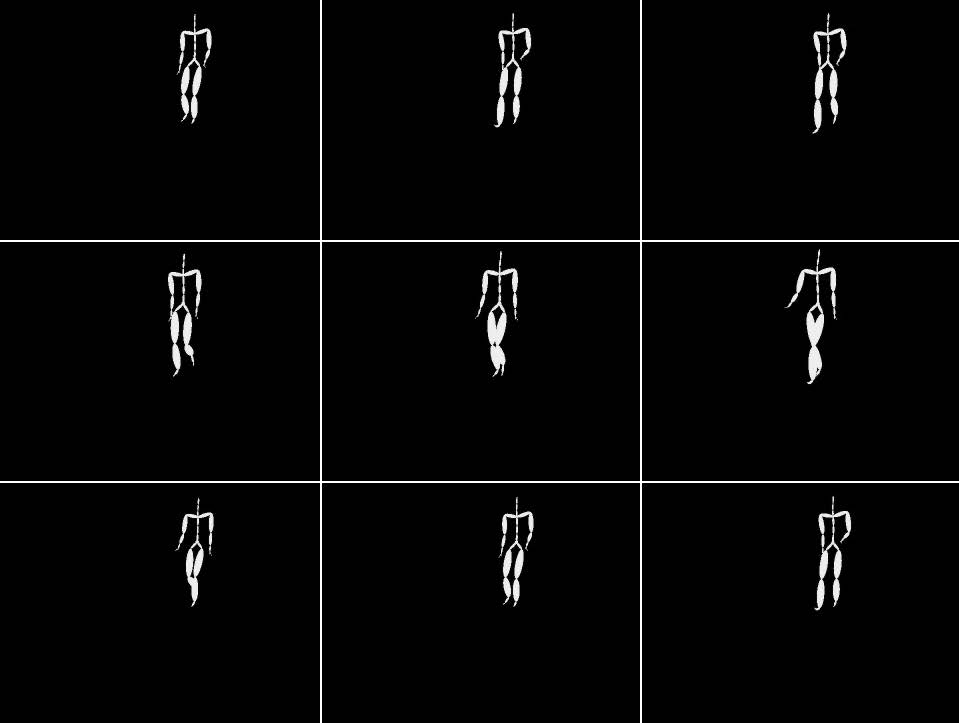
\includegraphics[width=0.5\textwidth]{walking.jpg}
		

	\end{frame}

	\begin{frame}
		\frametitle{Anomaly Detection: Types}
		
		\begin{itemize}
			\item Frames from other videos were inserted to produce an anomaly.
			\item Type 1: the object quickly changed the position.
			\item Type 2: the movements were similar, but different actions were performed.
		\end{itemize}
	
		\centering
		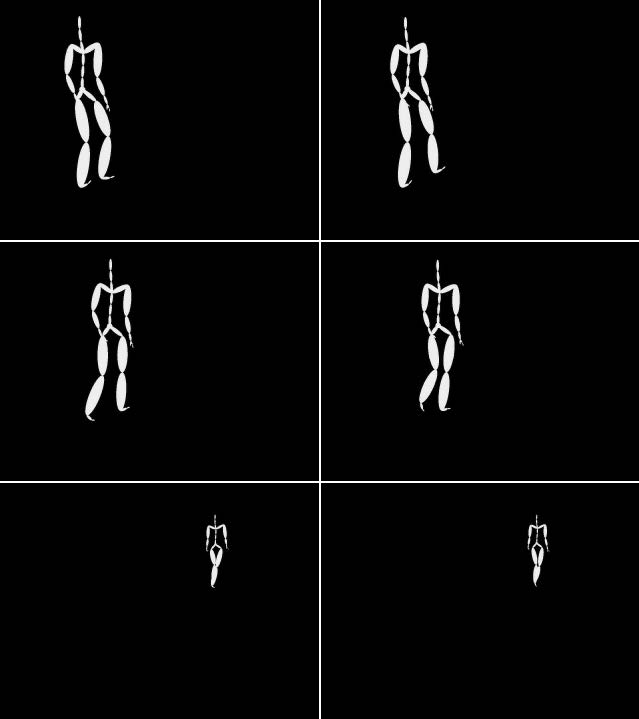
\includegraphics[width=0.3\textwidth]{anom1.jpg}
		\quad
		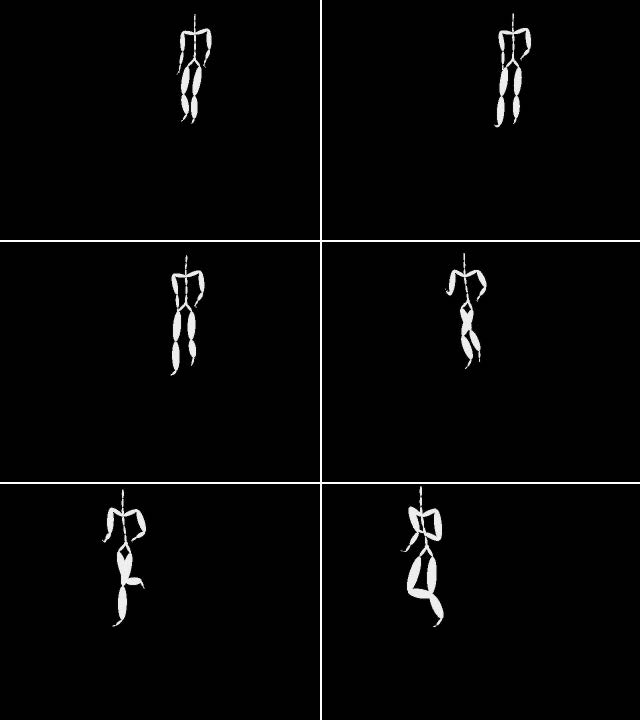
\includegraphics[width=0.3\textwidth]{anom2.jpg}

	\end{frame}

	\begin{frame}
		\frametitle{Schema of the processing}
		
		\begin{columns}
		\begin{column}{0.5\textwidth}
			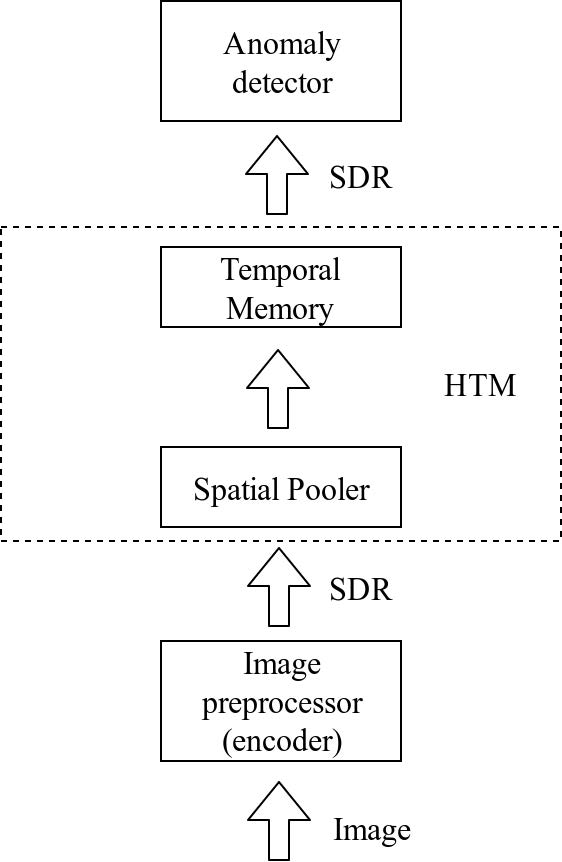
\includegraphics[width=0.8\textwidth]{schema.jpg}
		\end{column}
		\begin{column}{0.5\textwidth}
			Preprocessing:
			\begin{itemize}
				\item Image loading.
				\item Algorithms which control the sensor's movement around the image.
			\end{itemize}
			Score computing:
			\[
				score = \frac{\sum_{i=0}^n \left(ac_{expected}^{(i)}-ac_{real}^{(i)}\right)^2}{n}
			\]
			\nocite{*}
			\printbibliography[keyword={osipov}, resetnumbers=true]
		\end{column}
		\end{columns}
	\end{frame}

	\begin{frame}
		\frametitle{Experimental results}
		\centering
		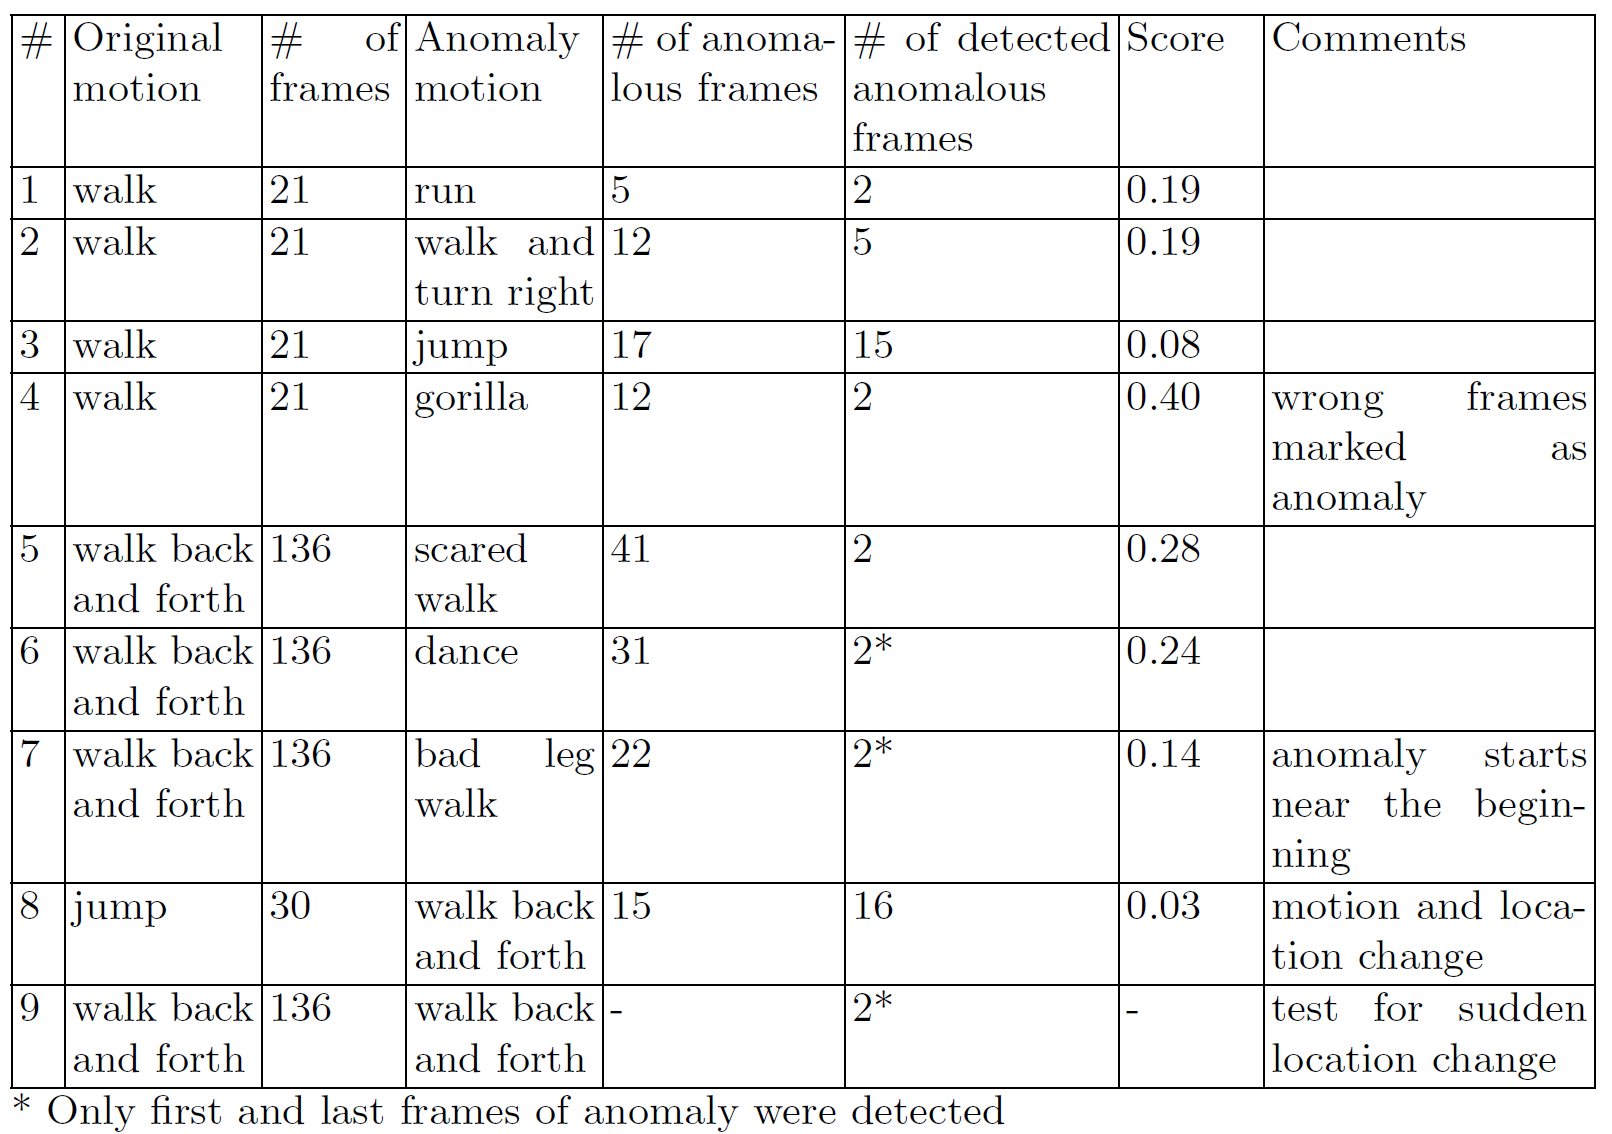
\includegraphics[width=0.7\textwidth]{table-res}
	\end{frame}

	\begin{frame}
		\frametitle{Experimental results}
		Extensions:
		\begin{itemize}
			\item A preprocessing step	between layers: performing a convolution of	temporal memory region's output with some function (kernel).
			\item Feedback: producing commands to a sensor's view which will move it accordingly, therefore focusing on different parts of the image. It will have an SDR of combined
			information as input: the output of higher level's temporal memory, the current
			frame of the video and reward.
		\end{itemize}
		\centering
		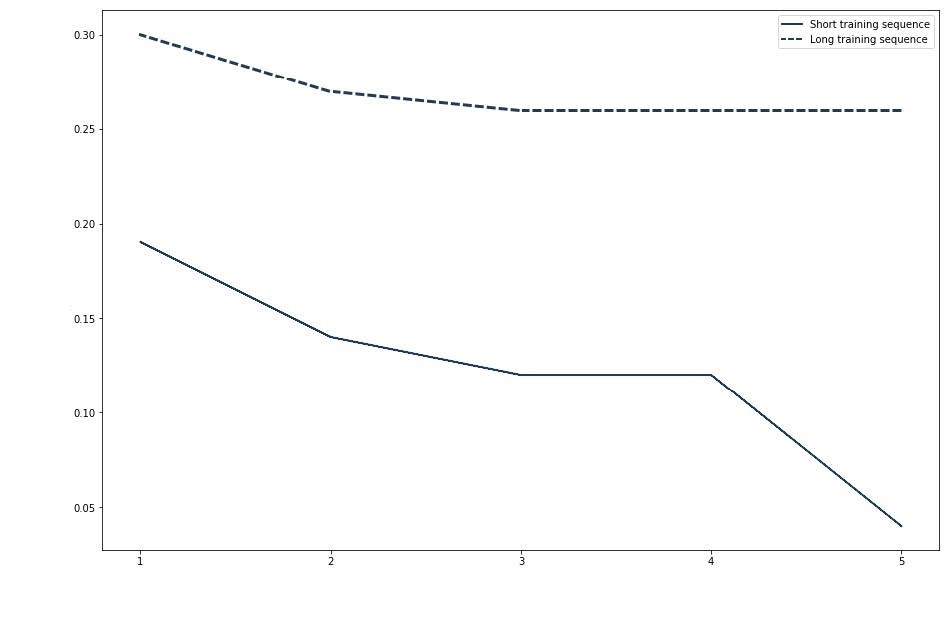
\includegraphics[width=0.45\textwidth]{layers-res1}
		\quad
		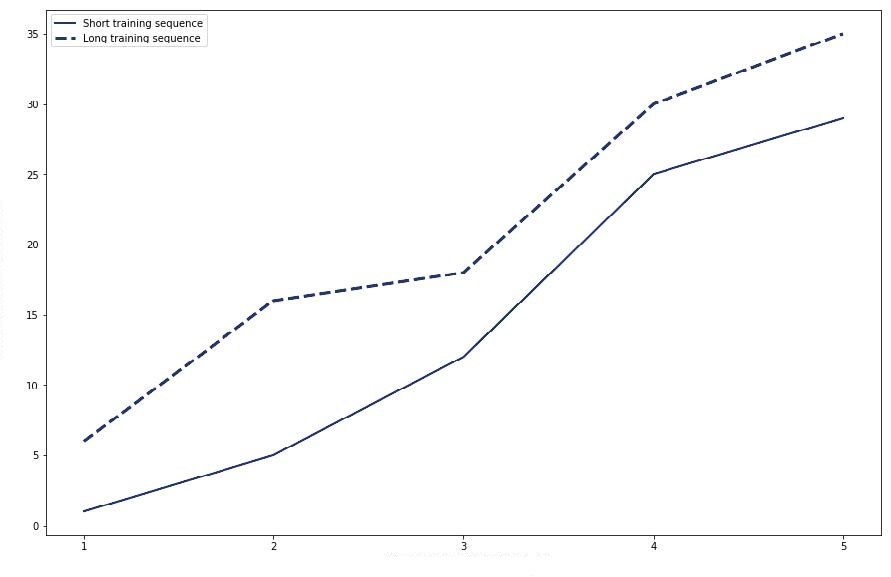
\includegraphics[width=0.45\textwidth]{layers-res2}
	\end{frame}

	\begin{frame}
		\frametitle{Experimental results}
		
		\centering
		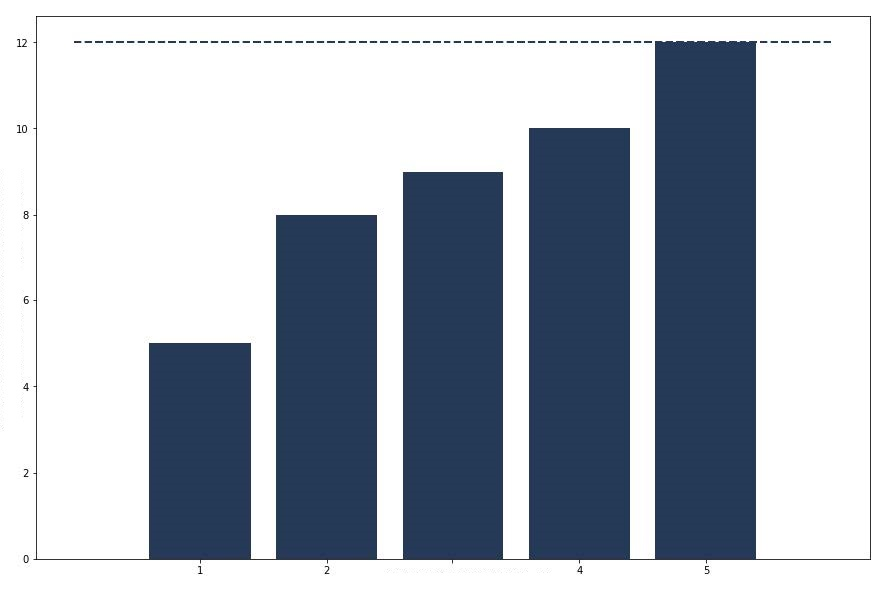
\includegraphics[width=0.45\textwidth]{layers-res3}
		\quad
		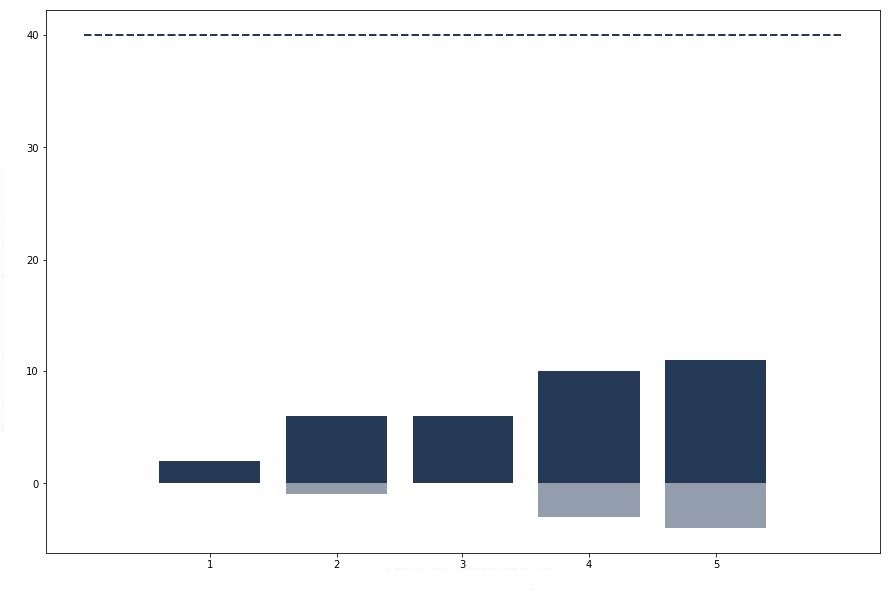
\includegraphics[width=0.45\textwidth]{layers-res4}
	\end{frame}

	\begin{frame}
	
		\centering
		\Huge
		Thank you for your attention!
		\normalsize
		\par\bigskip
		\par\bigskip
		\par\bigskip
		panov.ai@mipt.ru
	\end{frame}			
\end{document}
	
	
